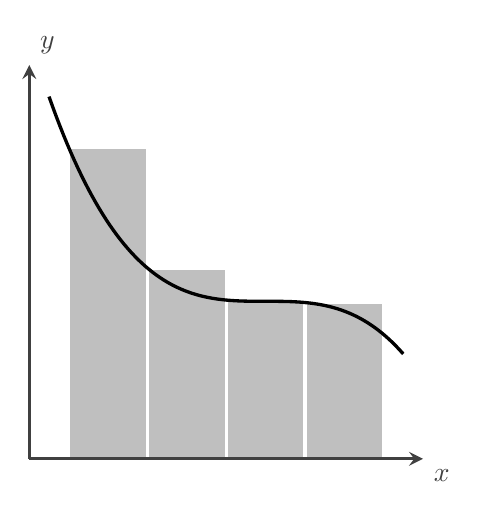
\begin{tikzpicture}[
    declare function={fone(\x)=((3-\x)^3)/8+2;}, 
  very thick, line join=round]

  % Draw squares
  \foreach [evaluate={\y=fone(\x);}] \x in {0.5,...,3.5}{
    \path [fill=black!25, draw=white] 
    (\x, 0) -- 
    (\x+1, 0) -- 
    (\x+1, \y) -- 
    (\x, \y) -- 
    cycle;
  }

  % Draw functions
  \draw [black, domain=0.25:4.75, samples=100, variable=\t] 
  plot (\t, {fone(\t)});

  % x-axis
  \draw [-stealth, black!75] (0,0) -- (5,0) node [below right] {$x$};

  % y-axis
  \draw [-stealth, black!75] (0,0) -- (0,5) node [above right] {$y$};


\end{tikzpicture}
